\section{Implementation}
\label{implementation}

The first CTFE First was created for the C-=-1 language, using out-of-the-box parser generator and backend.

\subsection{Interpreter data structures}

Data structures of the C-=-1 Interpreter have been designed ease of development and debugging in mind.
They are thus not particularly efficent.

\begin{figure}
	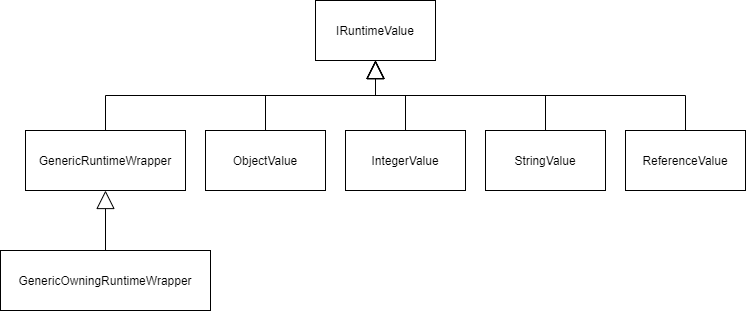
\includegraphics[width=8cm]{pictures/interpreter_data_structures_uml.png}
	\caption{Class diagram of C-=-1 interpreter data structures}
	\label{fig:interpreter_data_structures}
\end{figure}

Figure \ref{fig:interpreter_data_structures} contains a class diagram of most of the types used to represent values within C-=-1.




\subsection{Program semantic model}

\subsection{Backend interface}
\label{implementation/backend-interface}
